\documentclass{article}
\usepackage[utf8]{inputenc}
\usepackage[bulgarian]{babel}
\usepackage{graphicx}
\usepackage{titlesec}
\usepackage{biblatex}
\usepackage{amsmath}
\addbibresource{bibliography.bib}
\newcommand\tab[1][1cm]{\hspace*{#1}}
\graphicspath{ {images/} }

\title{РАЗРАБОТВАНЕ НА ПЛАТФОРМА ЗА 3D ВИЗУАЛИЗАЦИЯ БАЗИРАНА НА УЛТРАЗВУКОВА СИСТЕМА ЗА ПОЗИЦИОНИРАНЕ}

\author{Христо Христов}
\date{Юни 2017}

\begin{document}

\maketitle

\centerline{\large{Дипломна работа}}
\centerline{\large{Бургаски свободен университет}}

\tableofcontents

\pagebreak
\section{Въведение}

\subsection{Увод}
\tabНастоящата дипломна работа се фокусира върху разработване на платформа за тримерна визуализация на обекти в ограничен регион, използвайки измервателните възможности на ултразвук трансмитери и получатели. Използването на ултразвук за определянето на позицията на обекти в пространството, има потенциал да бъде употребявана в региони, в които GPS сигналът е прекалено слаб или заглушен [1].

\subsection{Цел}
\tabОсновната цел на настоящата дипломна работа е да се разработи платформа за тримерна визуализация, базирана на ултразвукова система за позициониране.

\subsection{Задачи}
За постигане на поставената цел е необходимо да бъдат изпълнени следните задачи
\begin{itemize}
    \item Да се изследва:
     на използване на ултразвуков сигнал за построяването на 3D картина в реално време и приложимите решения за този проблем.
    \itemДа се анализират :
    \begin{enumerate}
     \itemВъзможните ултразвукови предаватели и приемници, за да се определи, дали такава система би била удачна за нуждите на индустрията.
     \itemСложността на работата на системата и качеството на визуализацията на обектите.
    \end{enumerate}
    \itemДа се разработят:
    \begin{enumerate}
    \itemАлгоритъм за определяне на координатите на обектите от измеренията за разстояние, които приемниците и предавателите измерват.
    \itemСофтуерна програма за визуализация в 3D на определените координати.
    \end{enumerate}
    \itemДа се тества:
    \begin{enumerate}
    \itemРаботата на софтуерната програма в реални условия.
    Ограниченията на програмата спрямо броя на движещи приемници и стационарни предаватели.
    \end{enumerate}
\end{itemize}

\pagebreak
\section{Характеристика и сравнителен анализ на алгоритми за позициониране}

В настоящата глава се изследват ?? на брой различни алгоритъма за определяне на координатите на получатели на ултразвуков сигнал. Софтуерна имплементация е реализирана за следните алгоритми. \begin{enumerate}
    \item \ref{squares_algorithm}
\end{enumerate}

\subsection{Метод на най-малките квадрати} \label{squares_algorithm}

Изпозлвайки метода на най-малките квадрати представен в \cite{leastsq} се демонстрира намиране на решение чрез разширение на Теоремата на Питагор за 3D. За да се трансформира горната задача в математически модел е нужно да имаме anchor\cite{leastsq2}, което преставлява ориентировъчна точка в пространстовото, в което ще определяме координатитите. За anchor обект избираме позицията на първия получател във виртуалното пространство. Позицията в пространтовото на получателите е константно и е известно винаги.


\begin{equation} \label{pytEq}
   (x-x_i)^2 + (y-y_i)^2 + (z-z_i)^2=d_i^2
\end{equation}

Уравнение \ref{pytEq} описва взаимовръзката между разстоянието и координатите на два обекта. За да генерализираме уравнението, с индекс \textit{l} означаваме стойностите за anchor обекта. Чрез трансформация на уравнението се достига до следния запис:

\begin{equation} \label{pytEqTransformed}
  2 x (x_i - x_l) - 2 y (y_i - y_l) - 2  z  (z_i - z_l) = d^2_i - d^2_l - k_l + k_i
\end{equation}

За краткост в уравнение \ref{pytEqTransformed} променливата \textit{k} е означена като: 
\begin{equation} \label{kdesc}
    k_i= x^2_i + y^2_i + z^2_i
\end{equation}

Следното матрично уравнение служи за намиране на координатите:\\

\centerline{
    $
    2 \begin{bmatrix}
        (x_2-x_1) & (y_2 - y_1) & (z_2 - z_1)\\
        (x_3-x_1) & (y_3 - y_1) & (z_3 - z_1)\\
        (x_4-x_1) & (y_4 - y_1) & (z_4 - z_1)
    \end{bmatrix}
    $
    $
    \begin{bmatrix}
        x\\y\\z
    \end{bmatrix}
    $
    =
    $
    \begin{bmatrix}
        d^2_1 - d^2_2 - k_1 + k_2\\
        d^2_1 - d^2_3 - k_1 + k_3\\
        d^2_1 - d^2_4 - k_1 + k_4\\
    \end{bmatrix}\\
    $
}\\

Уравнението може да бъде решено от множество пакети за компютърна математика включително от MathNet Numerics \cite{numerics}.

\pagebreak

\subsection{Метод за следене използвайки ултразвук за увеличена реалност}

В документ \cite{vr} се описва система изградена от 4 получателя, които са позиционирани в ъглите на региона. Описани са 3 равнини [фиг. \ref{fig:planes}], които се използват за изчислението на координатите на точките. Това е еквивалентно на линеризиране на уравненията, за което в \cite{murphy} е споменато като метод, който не дава задоволителни резултати в реални условия.  Изчисленията на координатите се извършват с помощта на  Питагоровата теорема. За целта се използват  следните уравнения. \\

\centerline{
    \begin{equation}
        k=i+2
    \end{equation}
}

\centerline{
    \begin{equation} \label{22eq}
        \begin{bmatrix}
                $(x_i - x)^2 + y^2 = d_i_2$\\
                $(x_k - x)^2 + y^2 = d^2_k$
        \end{bmatrix}
    \end{equation}
}

\begin{figure}
    \centering
    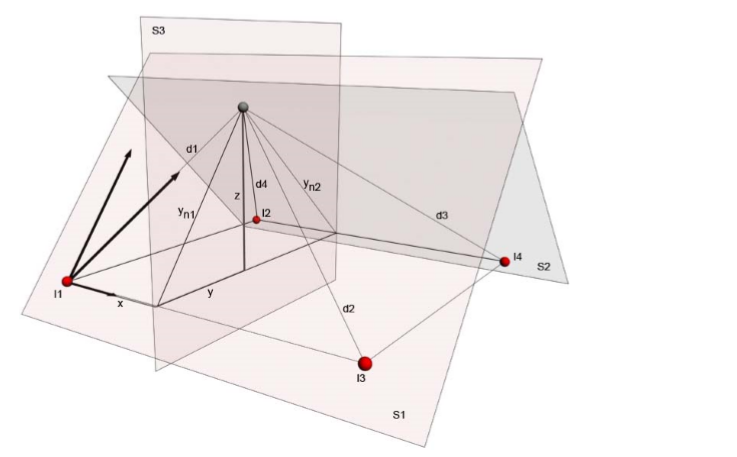
\includegraphics{planes}
    \caption{Равнините използвани за пресмятането на координатите}
    \label{fig:planes}
\end{figure}

\pagebreak

\subsection{Определяне на позиция в 3 измерения с помоща на трилатерация и приблизителни разстояния}

В документ \cite{murphy} е разработена система за следене на товарите в 3 измерения в мина чрез използване на трансмитери и получатели [фиг. \ref{fig:mine}]. Използвани са радио трансмитери. Разработен е специализиран лазер, който изчислява височината на товара, без който проблема за 3 измерения се е считал за нерешим. Проблем представляват разликите във височината и останалите измерения тъй като останалите измерения са в пъти по-големи в повечето случаи, както се вижда във фигура \ref{fig:initPos}, тъй като това тази разлика често води до изродени матрици.

\begin{figure}
    \centering
    \centerline{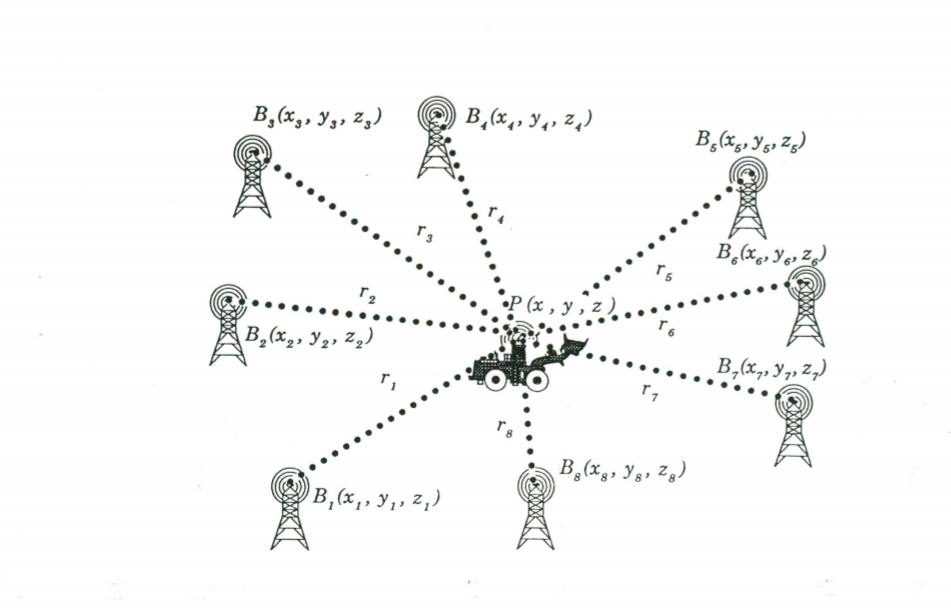
\includegraphics{dt1}}
    \caption{Разположение на получателите и предавателя в мина}
    \label{fig:mine}
\end{figure}

\begin{figure}
    \centering
    \centerline{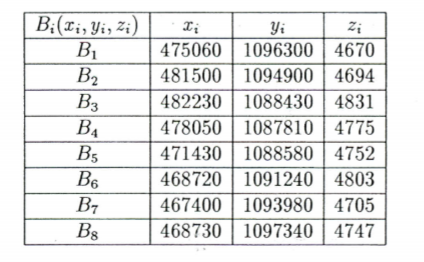
\includegraphics{MurphyInitialPositions}}
    \caption{Начално разположение на статичните получатели}
    \label{fig:initPos}
\end{figure}


\begin{equation}\label{circleEq}
    (x-x_i)^2 + (y-y_i)^2 +(z-z_i)^2=r_i^2
\end{equation}

Разглежда се възможността за съствяне система от \textit{N} на брой нелинейни уравнения използвайки формулата за сфера (уравнение \ref{circleEq}). Задачата се моделира като търсене на пресечни точки на N на брой сфери за всеки трансмитер.

Решението на гореспоменатата нелинейна система от уравнения \emph{се счита за неоптимално} тъй като полученото уравнение е нелинейно и е от висока степен. Когато разстоянията, които са измерени са точни, а не са приблизителни, линезирането на системата от уравнения е удачно. В този случай задачата се преобразува в търсенето на пресечната точка на няколко равнини. Системи с по-малко от тази бройка приемници се считат за неизползваеми. \\

Разглежда се метод за линеризация на уравненията, за който всяка измерена дистанция между трансмитер и получател се използва уравнението за сфера ( кръг в 2D ) ( уравнение \ref{circleEq} ). Методът за линеризация съвпада с този използван в секция \ref{squares_algorithm}. Тъй като има (n-1) уравнения, за долна граница се считат 4 бр. приемника.
\\

Разглеждат се няколко метода за работа с приблизителни разстояния

\begin{itemize}
    \item \strong{Линейни най-малки квадрати} \\ Този метод предоставя по-задоволителни резултати в сравнение с решаване на проблема чрез решение на задачата с линеризиране на уравненията, но не дава оптимални резултати, защото резултатите определят координатите с  грешка повече от 5 фута, което в ситуацията описана в статия \cite{murphy}, е недостатъчно като точност. Тъй като разстоянията са приблизителни се решава уравнение \ref{matrixeq}. Чрез минимизиране на сумата на квадратите на остатъците, уравнение \ref{nonNormalEq} води до уравнение \ref{normalEq}. \textit{[Noble and Daniel 1988]}
    
    \begin{equation} \label{matrixeq}
      A \vec{x} \approx \vec{b} 
    \end{equation}
    
    \begin{equation} \label{nonNormalEq}
        S = \vec{r}^T \vec{r} = (\vec{b} - A \vec{x})^T ( \vec{b} - A \vec{x})
    \end{equation}
    
    \begin{equation} \label{normalEq}
        A^T A \vec{x} = A^T \vec{b}
    \end{equation}
    
        
    Ако матрицата A в изразa $A^T A$ на уравнение \ref{normalEq} не е изродена се използва уравнение \ref{nonSing} , за да се намери решение на задачата.

    \begin{equation} \label{nonSing}
        \vec{x} = (A^T A)^{-1} A^T \vec{b}
    \end{equation}
    
    \item \strong{Нелинейни най-малки квадрати}
    
\end{itemize}


\strong{Резултати}

\begin{figure}
    \centering
    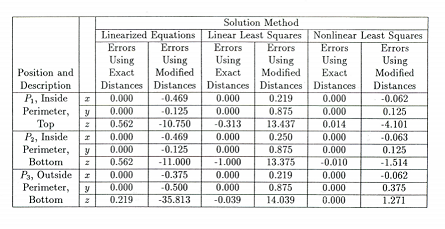
\includegraphics{murphyresults}
    \caption{Резултати при използване на различни методи за изчисление}
    \label{fig:murphyResults}
\end{figure}



Фигура \ref{fig:murphyResults} демонстрира резултатите при определянето на координатите. Най-добри резултати се получават при използването на нелинейни най-малки квадрати, а най-лоши при използването на линеризирани уравнения. Линейните най-малки квадрати водят до най-добри резултати, когато не съществува голяма разлика в стойностите на измеренията (x,y,z).

\pagebreak

\subsection{An Active Tracking System using IEEE 802.15.4-based Ultrasonic Sensor Devices}

В документ \cite{yonei} е имплементирана система за следене на обект в пространството използвайки IEEE 802.15.4 базирани ултразвукови сензори.
IEEE 802.15.4 се използва главно в безжичните сензорни мрежи заради ниската консумация на енергия и бързия обмен на информация между компонентите на системата \ref{fig:yoneiFig}. Системата съдържа 1 движещ се компонент. Координатите на движещия се компонент се изчисляват чрез използване на трилатерация.  Описани са 2 категории системи за обработка и изпращане на ултразвукови сигнали \cite{sysTypes}:

\begin{enumerate}
    \item Активни - движещите компоненти излъчват сигнал, а статичните компоненти получават сигнала и го обработват.
    \item Пасивни - движещите компоненти не излъчват сигнал, а получават сигнал, с който се определя разстоянието до различните получатели.
\end{enumerate}

\begin{figure}
    \centering
    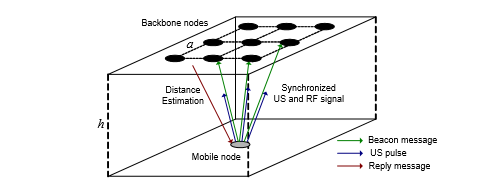
\includegraphics{yonei}
    \caption{Диаграма на разработената система}
    \label{fig:yoneiFig}
\end{figure}


Системата, която е разработена е класифицирана като активна.За коректно пресмятане на координатите на движещия се компонент се изискват измервания от поне 3 бр. статични компонента.



\pagebreak

\subsection{Позициониране чрез независими източници}

В документ \cite{bristolBeacons} се описва пасивна система [фиг. \ref{fig:bristolResults}], в която движещ се обект използва ултразвукови сигнали от няколко източника, за да определи позицията си в пространстовото. Движещия се обект използва разликите в периода на сигнала, което е форма на Доплеров ефект, за да определи своята позиция и скоростта си. Този подход е нов се счита за иновативен в измерването на разстоянието между различните обекти. Различава се от страндартния подход наречен time of flight (TOF), който се използва в текущата дипломна работа за измерване на разстоянията. Използвайки измервания на периода на получаване на сигнали, системата успешно идентифицира източника на даден сигнал. За да се гарантира, че приемника правилно ще идентифицира кой е текущия трансмитер, се използват подбрани периоди така че да не се получават конфликтни идентификации. За всеки трансмитер се изчислява, каква е промяната през изминалия период с помощта на зависимостта, която гласи, че изменението на пулса е пропорционално на разстоянието, което получателя е изминал през дадения период. Тази зависимост се изразява в уравнение \ref{prop}.

\begin{figure}
    \centering
    \centerline{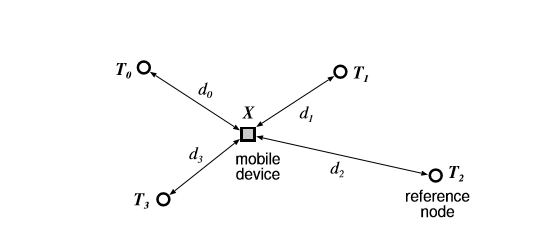
\includegraphics{bristolConfig}}
    \caption{Конфигурация на трансмитери и получатели}
    \label{bristolVis}
\end{figure}


\centerline{\begin{equation} \label{prop}
    \Delta d = v_s \Delta P_i
\end{equation}} \\

Системата се нуждае от поне 7 трансмитера, за да работи. 

За да се определи позицията на обекта се използва Kalman филтър с множество хипотези \cite{kalmanFilter}. За да се определи позицията се ипзолзва формула \ref{kalman}.

\centerline{\begin{equation} \label{kalman}
    ((X-T_i)/ (|X-T_i|)) * V = (\Delta P_i * v_s) / (P_i + \Delta P_i)
\end{equation}}\\

Чрез изпълняванет на много паралелни филтри се генерират хипотези за позицията на обекта в пространстовото. След протичането на този процес хипотезите се комбинират. В документ \cite{bristolBeacons} е решено хипотезите да бъдат комбинирани чрез осредняване на координатите. \\


\strong{Резултати} \\
Чрез използване на Kalman филтър са измерени резултатите изобразени на фиг. \ref{fig:bristolResults}

\begin{figure}
    \centering
    \centerline{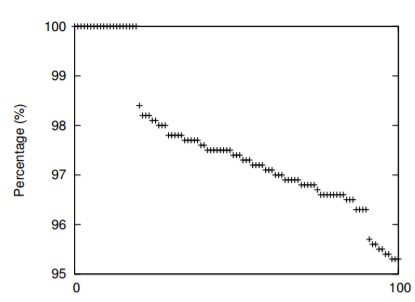
\includegraphics{bristolResults}}
    \caption{Качество на резултатите в проценти, при низходящо сортирани по дистанция данни}
    \label{fig:bristolResults}
\end{figure}

\pagebreak

\subsection{Kalman филтър} \label{kalmanSect}

В документ \cite{kalmanTutorial} се изследва приложимостта на Kalman филтър за определяне на дадена стойност при присъствие на несигурност или неточност в работните данни.

Популярността на Kalman филтър се базира на следните качества, които той притежава

\begin{enumerate}
    \item Добри практически резултати
    \item Удобен е за обработка на данни в реално време
    \item Лесна за реализация имплементация
    \item Измервателните уравнения не трябва да се инвертират
\end{enumerate}

Считайки нормално разпределение на грешката.
\pagebreak

\subsection{Обобщение}


\pagebreak

\pagebreak
\section{Избор и обосновка на технологии за разработка}
\subsection{Използвани технологии}


\begin{enumerate}
 \itemЗа разработката на приложението е използвана интегрираната среда за разработка на софтуер \textit{Visual Studio 2017}. 
 \itemИзползваният програмен език е \textit{C Sharp}. 
 \itemЗа визуализацията на примитиви в 3D е използвана библиотеката с отворен код \textit{Helix Toolkit 3D}. Позволява достъп до вече настроен viewport, както и някои базови за работата с 3D обекти функции – ротация, транслация и скалиране.
 
 \item \textit{XAML} е маркъп език за програмиране, който позволява лесно структуриране на визуална информация.
 
 \item \textit{WPF} е набор от инструменти, които улесняват разработката на софтуер за Windows базирани системи.
 
 \itemЗа олеснена работа със структурата от данни граф е използвана библиотеката с отворен код \textit{QuickGraph}. 
 
 \item \textit{LINQ} е език за манипулация на данни, имплементиран в .NET платформата.
 
 \item Math.NET Numerics е библиотека за линейна алгебра с отворен код.
 
 \item LaTeX е програмен език от високо ниво за създаване на документи с високо качество на шрифт и илюстрации използван широко в академичните документи \cite{latexUsage} \cite{latexUsage2}.
\end{enumerate}

\subsection{Обоснование за използвани технологии}

\begin{enumerate}
    \item Visual Studio предоставя мощна интегрирана среда за писане на код, компилиране, изпълнение, дебъгване (както за високо така и за машинно ниво), тестване на приложения, дизайн на потребителски интерфейс (форми, диалози, уеб страници, визуални контроли и други), моделиране на данни, моделиране на класове, изпълнение на тестове, пакетиране на приложения и стотици други функции. Могат да се добавят и плъгини, които повишават функционалността на почти всяко ниво – включително добавянето на поддръжка за source-control системи (като Subversion и Visual SourceSafe), добавяне на нови инструменти като редактори и визуални дизайнери за domain-specific languages или инструменти за други аспекти (като например: Team Foundation Server, Team Explorer). \cite{vs}. Visual Studio предлага удобен интерфейс за разработка на XAML базирани интерфейси. \ref{vsXAML}
    
    \item C Sharp е широкоприет програмен език, които заимства от различни парадигми в програмирането - функционално, обектно-ориентирано и т.н. Разработен е от Microsoft, което позволява лесна интеграция с останалите инструменти, които се използват в настоящата дипломна работа. C Sharp се счита за 5-тия най-популярене зик за програмиране според класацията на TIOBE. [фиг. \ref{fig:prog}]
    
    \item XAML e декларативен маркъп език използван за иницализиране на структурирани стойности и обекти. Използва се за оформление на структурата на софтуерни приложение. Разработен е от Microsoft и е единственият подържан маркъп език, който се подържа от платформата WPF. В настоящата дипломна работа, той се използва, за да се структурира визуално информацията използвана в софтуерната програма, която бе разработена.
    
    \item WPF ( Windows Presentation Foundation ) \cite{wpf} е набор от инструменти, които олесняват разработката на Windows Desktop приложения Използва се за главно за разработка на приложения за персоналния компютър, но може да бъде използван и в уеб среда. Често е предпочитан пред останалите варианти заради стабилността на инструментите и това че разработвания софтуер е независим от интернет връзка. Той подържа работа с 3D примитиви използвайки Direct X \cite{wpfUsage}. WPF е менажиран слой, който надгражда над базовите програмни интерфейси на Windows [фиг. \ref{fig:wpf}].
    
    \item Helix Toolkit надгражда вградените в WPF функционалности за работа с 3D обекти. Въпреки, че не може да се сравнява по мощност с напредналите инструменти за разработка на 3D модели, Helix Toolkit съдържа достатъчно функционалности, за да бъде достатъчна за работа с обекти в 3D. Съдържа оптимизирани имплементации на често използвани операции обработката на визуална информация ( скалиране , ротация и транслация). Съдържа помощни обекти, които позоволяват да се упражнява контрол над камерата. Съдържа помощни функции за контрол над осветлението във виртуалното пространство. \cite{helix}
    
    \item QuickGraph предлага стабилни имплементации на структурата от данни граф за платформата за разработка .NET. Това включва насочен/ненасочен граф. Имплементирани са често използвани алгоритми като търсене в дълбочина, търсене в дълбочина , A* търсене и т.н. \cite{quickgraph}.
    
    \textit{BidirectionalGraph<V,E>} е конкретната имплементация на граф използвана в проекта.  Тя представлява неориентиран граф, Използва се, за да се репрезентират обектите като върхове, а разстоянията измерени между обектите като дъги между върховете. Два обекта са свързани с не ориентирана дъга с тегло равно на разстоянието между двата обекта, ако няма измерение на разстоянието между обектите то тогава дъга между двата върха няма.
    
    \item LINQ (Language Integrated Query) е лесен и удобен начин да се манипулират данни в .NET базирани софтуерни приложения \cite{linq}. 
    
    \item Math.NET Numerics предлага методи и алгоритми за изчисления в науката, инженерните сфери и всекидневния живот. Покрива различни теми като -специални функции, линейна алгебра, статистически модели, случайни числа, интерполацич, интегриране, регресия, апроксимация на функции и бърза трансформация на Фурие [ FFT ] \cite{numerics}
    
    \item LaTeX  
    
    \itemЗа тестване на програмата в реални условия са използвани 4 бр. ултразвуков трансмитери и 1 бр. ултразвук получател, с производител : Hexamite. Устройствата са предоставени от др. Димитър Минчев

    
\end{enumerate}


\begin{figure}
    \centering
    \centerline{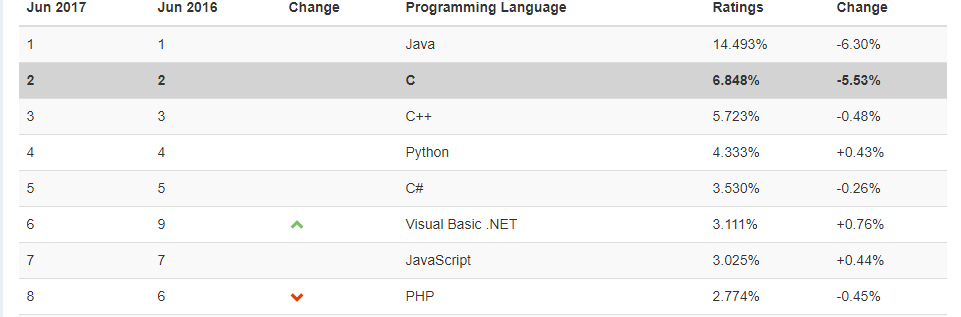
\includegraphics{programmingLanguage}}
    \caption{Езици за програмиране сортирани низходящо по популярност}
    \label{fig:prog}
\end{figure}


\begin{figure}
    \centering
    \centerline{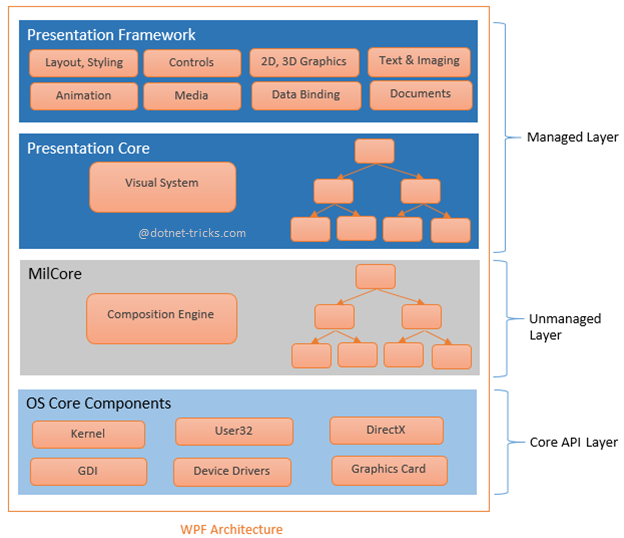
\includegraphics{wpfarchitecture}}
    \caption{Архитектура на набора от инструменти WPF}
    \label{fig:wpf}
\end{figure}

\begin{figure}
    \centering
    \centerline{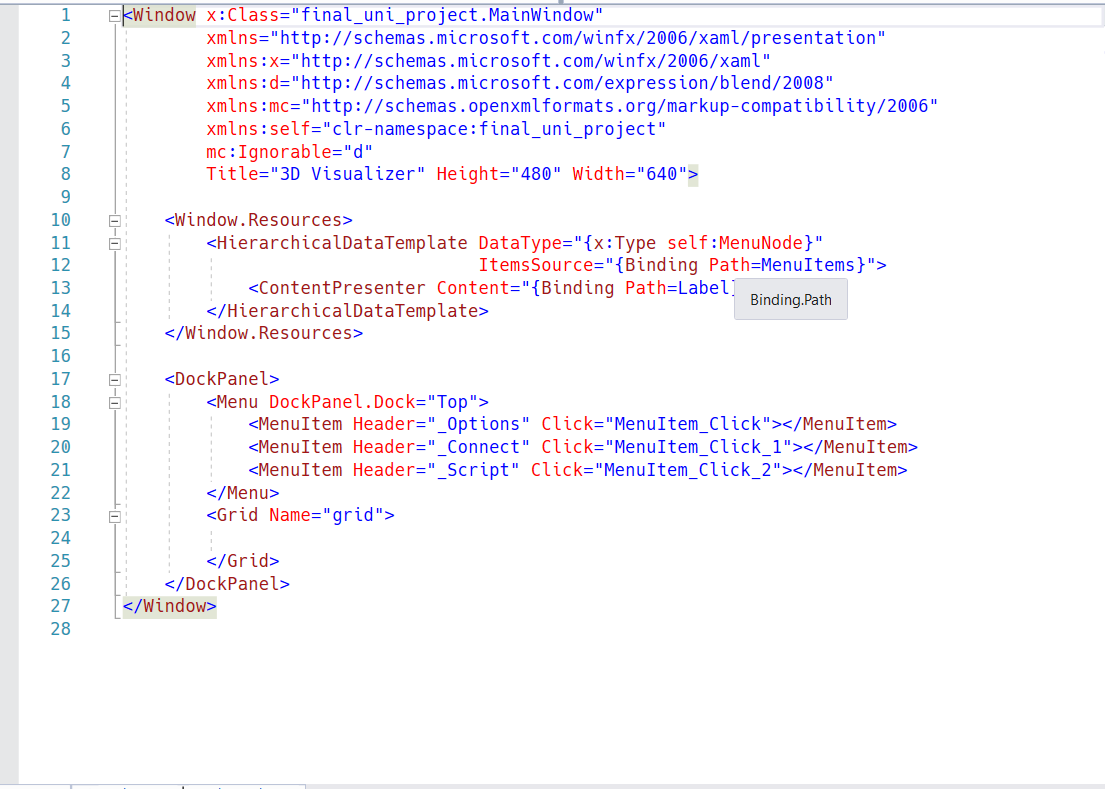
\includegraphics{xaml}}
    \caption{Разработка на XAML базирани приложения във Visual Studio}
    \label{vsXaml}
\end{figure}

\subsection{Обобщение}
Изборът на удачни технологии за разработка на софтуерен проект е една от най-важните стъпки в реализирането на проект \cite{technologiesImportance}. Правилния избор на технологии води до намален брой проблеми при разработката и действието на програмата, тъй като някой технологии статистически погледнато водят до по-малко проблеми \cite{langResearch}. В повечето случай тези технологии водят до по-малък обем на разработения софтуер, тъй като множество изследвания показват корелация между обема на софтуерните проекти и броят на бъгове в софтуерната програма \cite{bugsToLength}.

\pagebreak
\section{Разработване на платформа за 3D визуализация базирана на ултразвукова система за позициониране}
\subsection{Архитектура на софтуерна програма}
Всяка софутерна програма изисква разработката на интерфейс, чрез който потребителя може да комуникира със програмата. Софтуерната програма е съставена от 4 модула, които комуникират помежду си, някои, от които имат визуална част, а други - не.
За разработката на софтуерната програма са използвани множество от практики за дизайн (design patterns), което позволява лесната поддръжка на софтуера за бъдеще \cite{patterns}.Имплементацията на модулите е реализирана чрез използването на широкоизползваната практика за дизайн - MVVM \cite{mvvm}. Предишната прекитка, предлага ясно разпределение между отговорностите на различните части на кода т.е код, които отговаря за логически операции не е свързан с код, който отговаря за обратната връзка между двете. Прадлага лесен начин за синхронизиране между логическата и визуалната част на дадена софтуерна програма чрез използване на "One way data binding" и "Two way data binding" похватите \cite{dataBinding}.

\begin{figure}
    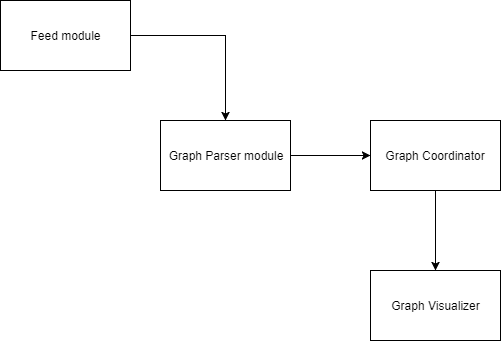
\includegraphics{modules}
    \caption{Архитектура на софтуерната програма}
    \label{fig:architecture}
\end{figure}

\begin{itemize}
    \item Options модул, който предлага начин за модифициране на различни настройки свързани с начина на изобразяване на обектите и тяхната начална конфигурация.
    \item Feed  модул, който има за отговорност да захранва с данни останалите модули с граф, който за всяка точка съдържа разстояниято между точката и всички останали точки. Ако разстоянието между две точки не може да бъде измерено то тогава разстоянието се означава с специален флаг поле, което е дефинирано като -безкрайност.
    \item Graph Parser модул, който има за цел да обработи информацията, която ‘Feed’ модулът изпраща и да я трансформира в друг граф – който държи информацията във върхове и дъги. Върховете и 
    дъгите съдържат информация, която помага за визуализацията на графа в 3D.
    \item Graph Coordinator модул, който има за цел да определи -координатите в пространството на всички обекти, които се съдържат в графа, който се получава в резултат на стъпка 2 (Graph Parser). Координатите се определят чрез система от линейни уравнения, които считат, че началната позиция на стационарните обекти е (0,0,0) - в един от ъглите на мястото, в което же бъдат следяни обектите.
    \item Graph Visualizer модул, който има за цел да използва графа, чиито координати са били вече определени от Graph Coordinator и да ги визуализира по удачен начин в 3 измерения.

\end{itemize}

\pagebreak

\subsection{Модул за опции}
Разработен е модул за опции, които позволява лесен контрол над началното разположение на статичните получатели в пространтвото. Модулът може да бъде използван чрез кликане на "Options" полето [фиг \ref{fig:options}]. Модулът изобразява презададен брой статични точки, чиито координати могат да бъдат зададени от потребителя на софтуерната програма. 

\begin{figure}
   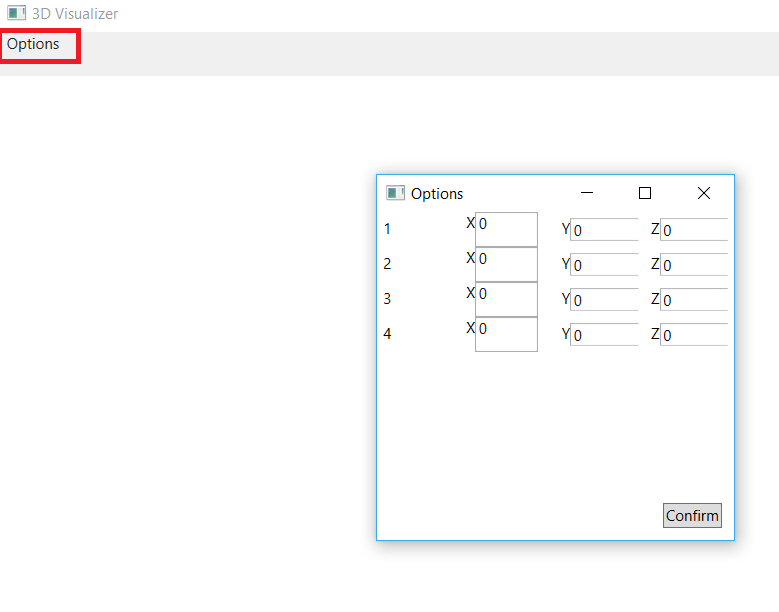
\includegraphics{OptionsLocation}
    \caption{Меню за опции}
    \label{fig:options}
\end{figure}

\pagebreak

\subsection{Feed модул}
Feed модулът има за цел да създаде граф, който съдържа дистанциите от всяка точка до всяка друга. Нуждата от възможност за лесна и бърза смяна между двата подхода наложи създаването на модула.\\\\
В процеса на работа бяха изградени 2 различни начина за получаване на данните от ултразвук трансмитери към ултразвук получатели. 
\begin{enumerate}
    \itemДанните се получават директно от физическите обекти. Стандартното измерване се случва чрез получаване на данните през сериен порт. Данните се предоставят от ултразвукови трансмитери и получатели в специален формат, който бива преобразуван към граф, съдържащ разстоянията между различните точки.
    \itemДанните биват генерирани чрез компютърен модел. Компютърния модел се състои от генератор на дистанции, който симулира движението на реален обект. Това се постига чрез манипулация на дистанцията между двойка (движещ,недвижещ) обект в пространството с константна стойност на определен интервал. Добавен е елемент на случайност, който позволява да се придаде по-реалистичен вид на движението на обектите.
\end{enumerate}

\pagebreak

\subsection{Graph Parser модул}
Graph Parser модулът има за цел да използва графа генериран от Feed модулът, за да създаде граф на свързаност, който съдържа
\begin{enumerate}
\itemВърхове, които представляват движещи/недвижещи се обекти 
\itemДъги, свързващи върховете, които означават съществуването на свързаност между
даден връх и друг връх.
\end{enumerate}

\pagebreak

\subsection{Graph Coordinator модул}
Целта на Graph Coordinator модула е да определи координатите в 3D на построения граф. Тази операция се извършва чрез минимизиране на бройката на възможните позиции използвайки система от уравнения. Всички възможни позиции се намират на радиус с дължина R (равен на дистанцията получена от сензора) на сфера. Задачата се трансформира:\\

\textit{За всеки получател се образуват K сфери (K=броя на трансмитерите), като сфера $x_i$ се центрира в позицията на на трансмитер с индекс $i$, а радиусът и е равен на измерената стойност за разстоянието между двата обекта. За да получим еднозначно решение ние трябва да елиминираме всички възможни позиции освен една. Всички решения на задачата за даден получател се намират на пресечния регион на всички сфери за дадения получател. Търси се такава конфигурация на позициите на всички получатели така че назначените позиции да не са в конфликт и броят на възможни решения за всяка позиция да е минимален.}\\\\

В 2D намирането на решения е лесно, поради следните причини:

\begin{enumerate}
    \itemБроят на пресечните точки на сферите при оптимално* позициониране на сензорите лесно може да бъде сведено до еднозначно решение.

    \itemВ 2-D пресечните точки на окръжностите са точки. В 3D пресечните точки се описват от 3D фигура. Това лесно може да бъде видяно на фигура \ref{spheres}.
\end{enumerate}

\begin{figure}
    \centerline{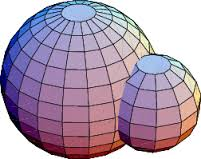
\includegraphics{spheres}}
    \caption{Пресечната точка на сфери в 3D е 3D регион от точки}
    \label{spheres}
\end{figure}

\pagebreak

\subsection{Graph Visualizer модул}
Целта на Graph Visualizer модула е да използва графа, чиито координати са били вече определени от Graph Coordinator и да ги визуализира по удачен начин в 3 измерения.


\subsection{Обобщение}
Разработена е архитектура за софтуерно решение за платформа за визуализация на ултразвукови компоненти в 3 измерения. Архитектурата на софтуерната програма е се състои от 5 модула, от които 1 е независим от останалите (модул за опции). 

\pagebreak
\section{Резултати, перспективи за развитие и заключение}
\subsection{Резултати}

В настоящата дипломна работа е разработена система за 3D визуализация на движещи се и стационарни обекти, чрез използването на ултразвук за измерване на дистанцията между стационарни обекти наречени предаватели на сигнал и потенциално движещи се обекти наречени получатели на сигнал. Системата е тествана в реални условия чрез използването на 4 стационарни ултразвукови предавателя и един движещ се приемник. Разработени са възможни сценарии за използване на системата в индустрията и извън нея. Системата е сравнена с вече съществуващи на пазара системи и са изкарани изводи, които сравняват качествата и недостатъците им.

Изследват се възможностите за визуализация на системи с много движещи се и стационарни обекти и ограниченията, които биват наложени от разработената технология спрямо броя на обектите, които биват изобразявани.

Системата е разработена с най-новите практики в софтуерното инженерство, които позволяват бързо и лесно да се модифицират различни модули от приложението без това да създава проблеми в останалите модули и е достъпна да бъде използвана с цел допълнително развитие.

\subsection{Перспективи за развитие}
Разработената система може да бъде развита с цел комерсиална употреба като пълноправен софтуерен продукт, както и да бъде използвана за персонални цели. Подобна система се използва в \cite{vr} за целите на ориентация във увелиячената реалност. Софтуерната имплементация може да бъде разширена с допълнителни модули за анализ на данните. Текущата имплементация приема, че данните получени от ултразвук трансмитери и получатели са валидни. Имплементацията може да бъде разширена като се добавят филтри за смущение и невалидна информация. В текущата статия скоростта на движението на ултразвука във въздуха се счита за константа, но в реални условия тя е пряко зависима от температурата на стаята \cite{vr}.

\subsection{Заключение}
Разработена е система за 3D визуализация на компонентите на система, която използва утразвук за измерване на разстоянията между компонентите на системата. Сравнени са предимствата и недостатъците на съществуващи системи използвани в индустрията. Изследвани са начини за определяне на координатите на компонентите във виртуалното пространство. Имплементирана е софтуерна програма, която извършва визуализацията на компонентите и са изследвани достъпните инструменти, които имат потенциала да помагат в разработката на подобен продукт.

\subsection{Приложение}

\begin{itemize}
    \item Образуване на входящ граф от дистанции
    \item Образуване на работен граф
    \item Определяне на координатите на компонентите на графа
    \item Изобразяване на резултата
\end{itemize}

\pagebreak
\section{Лицензи}
\subsection{Helix Toolkit 3D}
\begin{itemize}
    \item Връзка към лиценза : https://github.com/helix-toolkit/helix-toolkit/blob/develop/LICENSE
    \item Автор : Oystein Bjorke
\end{itemize}

\subsection{QuickGraph}
\begin{itemize}
    \item Връзка към лиценза: https://quickgraph.codeplex.com/license
    \item Автори : https://quickgraph.codeplex.com/team/view
\end{itemize}


\printbibliography

\end{document}
